\section{Projeção de pontos 3D em imagens 2D}

\subsection{Estimação da pose e separação dos pontos}

O experimento de \texttt{project.py} utiliza os parâmetros já salvos e três
fotografias inéditas por câmera, de \texttt{project\_test/}, sem recalibrar as
câmeras. O mesmo procedimento é aplicado às fotografias da calibração para
comparação. Os 16 cantos do tabuleiro têm coordenadas conhecidas
$\mathbf{P}_{r,c}=(3{,}1c,\,3{,}1r,\,0)$~cm, com $r,c\in\{0,1,2,3\}$.
O índice é $4r+c$, com a coluna variando primeiro, conforme a ordenação usada
na calibração. A origem está no canto de índice zero. Essas coordenadas
pertencem ao referencial local do tabuleiro, e não a um sistema global.

Após a detecção e o refinamento dos cantos, 12 correspondências entre pontos
3D e posições 2D observadas estimam a rotação e a translação do tabuleiro por
uma única chamada a \texttt{cv2.solvePnP()}, no modo
\texttt{SOLVEPNP\_ITERATIVE}. A pose transforma o referencial do tabuleiro no
referencial da câmera~\cite{opencv-calib3d}. A seleção é determinística: os
índices $0$, $3$, $12$ e $15$, situados nos quatro extremos da grade interna,
ficam reservados; os outros 12 se distribuem pelas quatro linhas e colunas.
Os pontos reservados não entram no \texttt{solvePnP()} nem em um refinamento
posterior da pose.

Com a pose estimada, \texttt{cv2.projectPoints()} calcula as coordenadas previstas
dos quatro pontos reservados, usando a matriz intrínseca, os coeficientes de
distorção e os vetores de rotação e translação. A comparação é feita no domínio
da fotografia original: não são usadas as imagens corrigidas por
\texttt{undistort.py}, pois a projeção já incorpora a distorção. O procedimento
é repetido por fotografia, com 12 pontos de pose e quatro de validação.

\subsection{Métricas e resultados}

Se $(u_i,v_i)$ é a posição observada e $(\hat{u}_i,\hat{v}_i)$ a posição
prevista, o erro individual, em pixels, é
\begin{equation}
e_i=\sqrt{(u_i-\hat{u}_i)^2+(v_i-\hat{v}_i)^2}.
\label{eq:error}
\end{equation}
Para os $N$ pontos de validação de uma câmera, calculam-se
\begin{equation}
\bar e=\frac{1}{N}\sum_{i=1}^{N}e_i,\qquad
\mathrm{RMSE}=\sqrt{\frac{1}{N}\sum_{i=1}^{N}e_i^2},\qquad
e_{\max}=\max_i e_i.
\label{eq:metrics}
\end{equation}
A média descreve o desvio típico, o RMSE atribui maior peso aos erros elevados
e o máximo registra o maior desvio individual. Todas as métricas globais
utilizam os erros ponto a ponto; não se faz a média dos RMSEs por imagem.

As três fotografias inéditas de cada câmera foram processadas sem falhas de
detecção ou estimação da pose, totalizando 12 pontos de validação por câmera.
Os resultados estão em \texttt{projections/tests/summary.txt} e
\texttt{points.csv}. A Tabela~\ref{tab:projection} também apresenta a referência
obtida nas 22 fotografias de calibração da câmera 1x e nas 20 da câmera 0,5x,
com 88 e 80 pontos reservados, respectivamente. As métricas de cada conjunto
foram calculadas separadamente, sem excluir erros elevados.

\begin{table}[H]
  \centering
  \caption{Erros de projeção em pixels: fotografias da calibração e teste inédito.}
  \label{tab:projection}
  \begin{tabular}{llrrrr}
    \toprule
    Câmera & Conjunto & Imagens & Média & RMSE & Máximo\\
    \midrule
    1x & Calibração & 22 & 1,121 & 1,575 & 5,121\\
    1x & Teste inédito & 3 & 2,839 & 4,061 & 9,162\\
    \midrule
    0,5x & Calibração & 20 & 2,112 & 2,563 & 6,119\\
    0,5x & Teste inédito & 3 & 2,418 & 3,060 & 6,821\\
    \bottomrule
  \end{tabular}
\end{table}

As Figuras~\ref{fig:projection1} e~\ref{fig:projection05} apresentam fotografias
inéditas das duas câmeras, com detalhe da região do tabuleiro. Os marcadores
são maiores apenas para facilitar a leitura; as distâncias da
Equação~\eqref{eq:error} foram calculadas com coordenadas de subpixel. Como os
desvios são pequenos na escala das figuras, observações e projeções podem
aparecer quase sobrepostas.

\begin{figure}[H]
  \centering
  \captionsetup{justification=raggedright,singlelinecheck=false}
  \begin{minipage}[t]{0.48\linewidth}
  \centering
  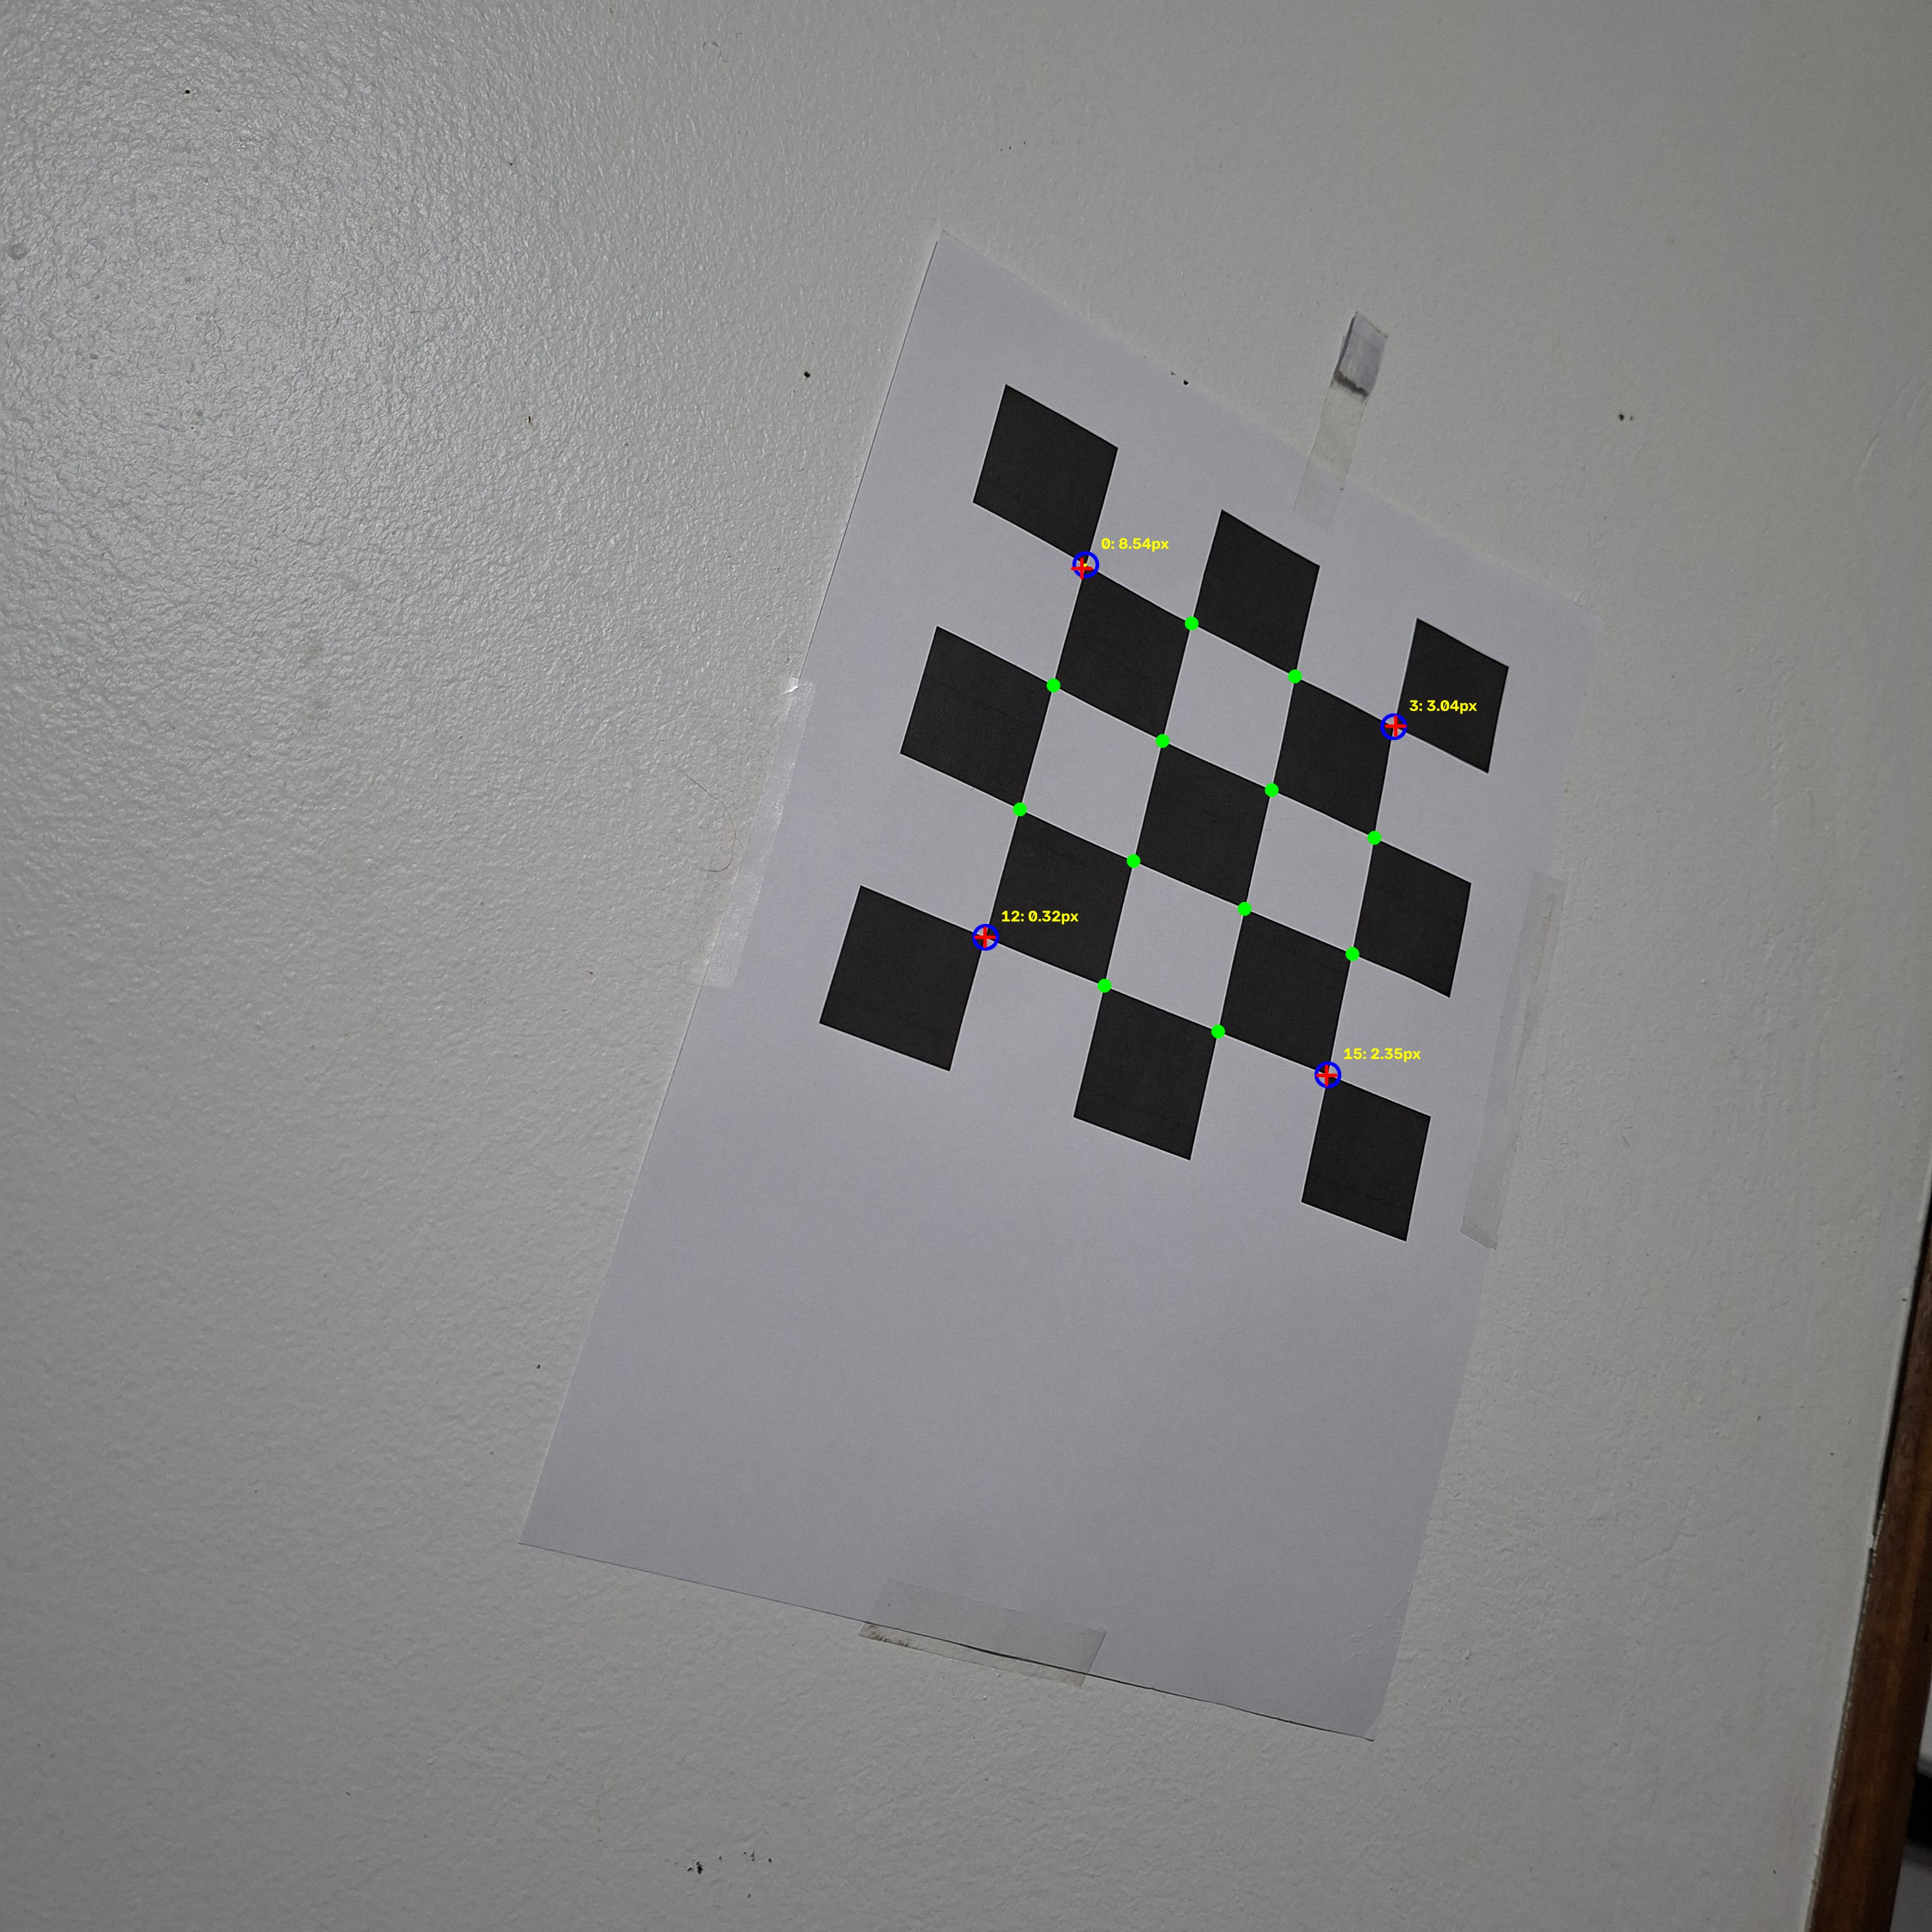
\includegraphics[height=5.5cm,trim=1325bp 1078bp 584bp 674bp,clip]{projection-cam1.jpg}
  \caption{Câmera 1x, fotografia inédita \texttt{001.jpg}. Verde: pose;
  azul: observações reservadas; vermelho: projeções. Amarelo: conexões e
  rótulos de erro. Média nesta imagem: $3{,}562$~px.}
  \label{fig:projection1}
  \end{minipage}\hfill
  \begin{minipage}[t]{0.48\linewidth}
  \centering
  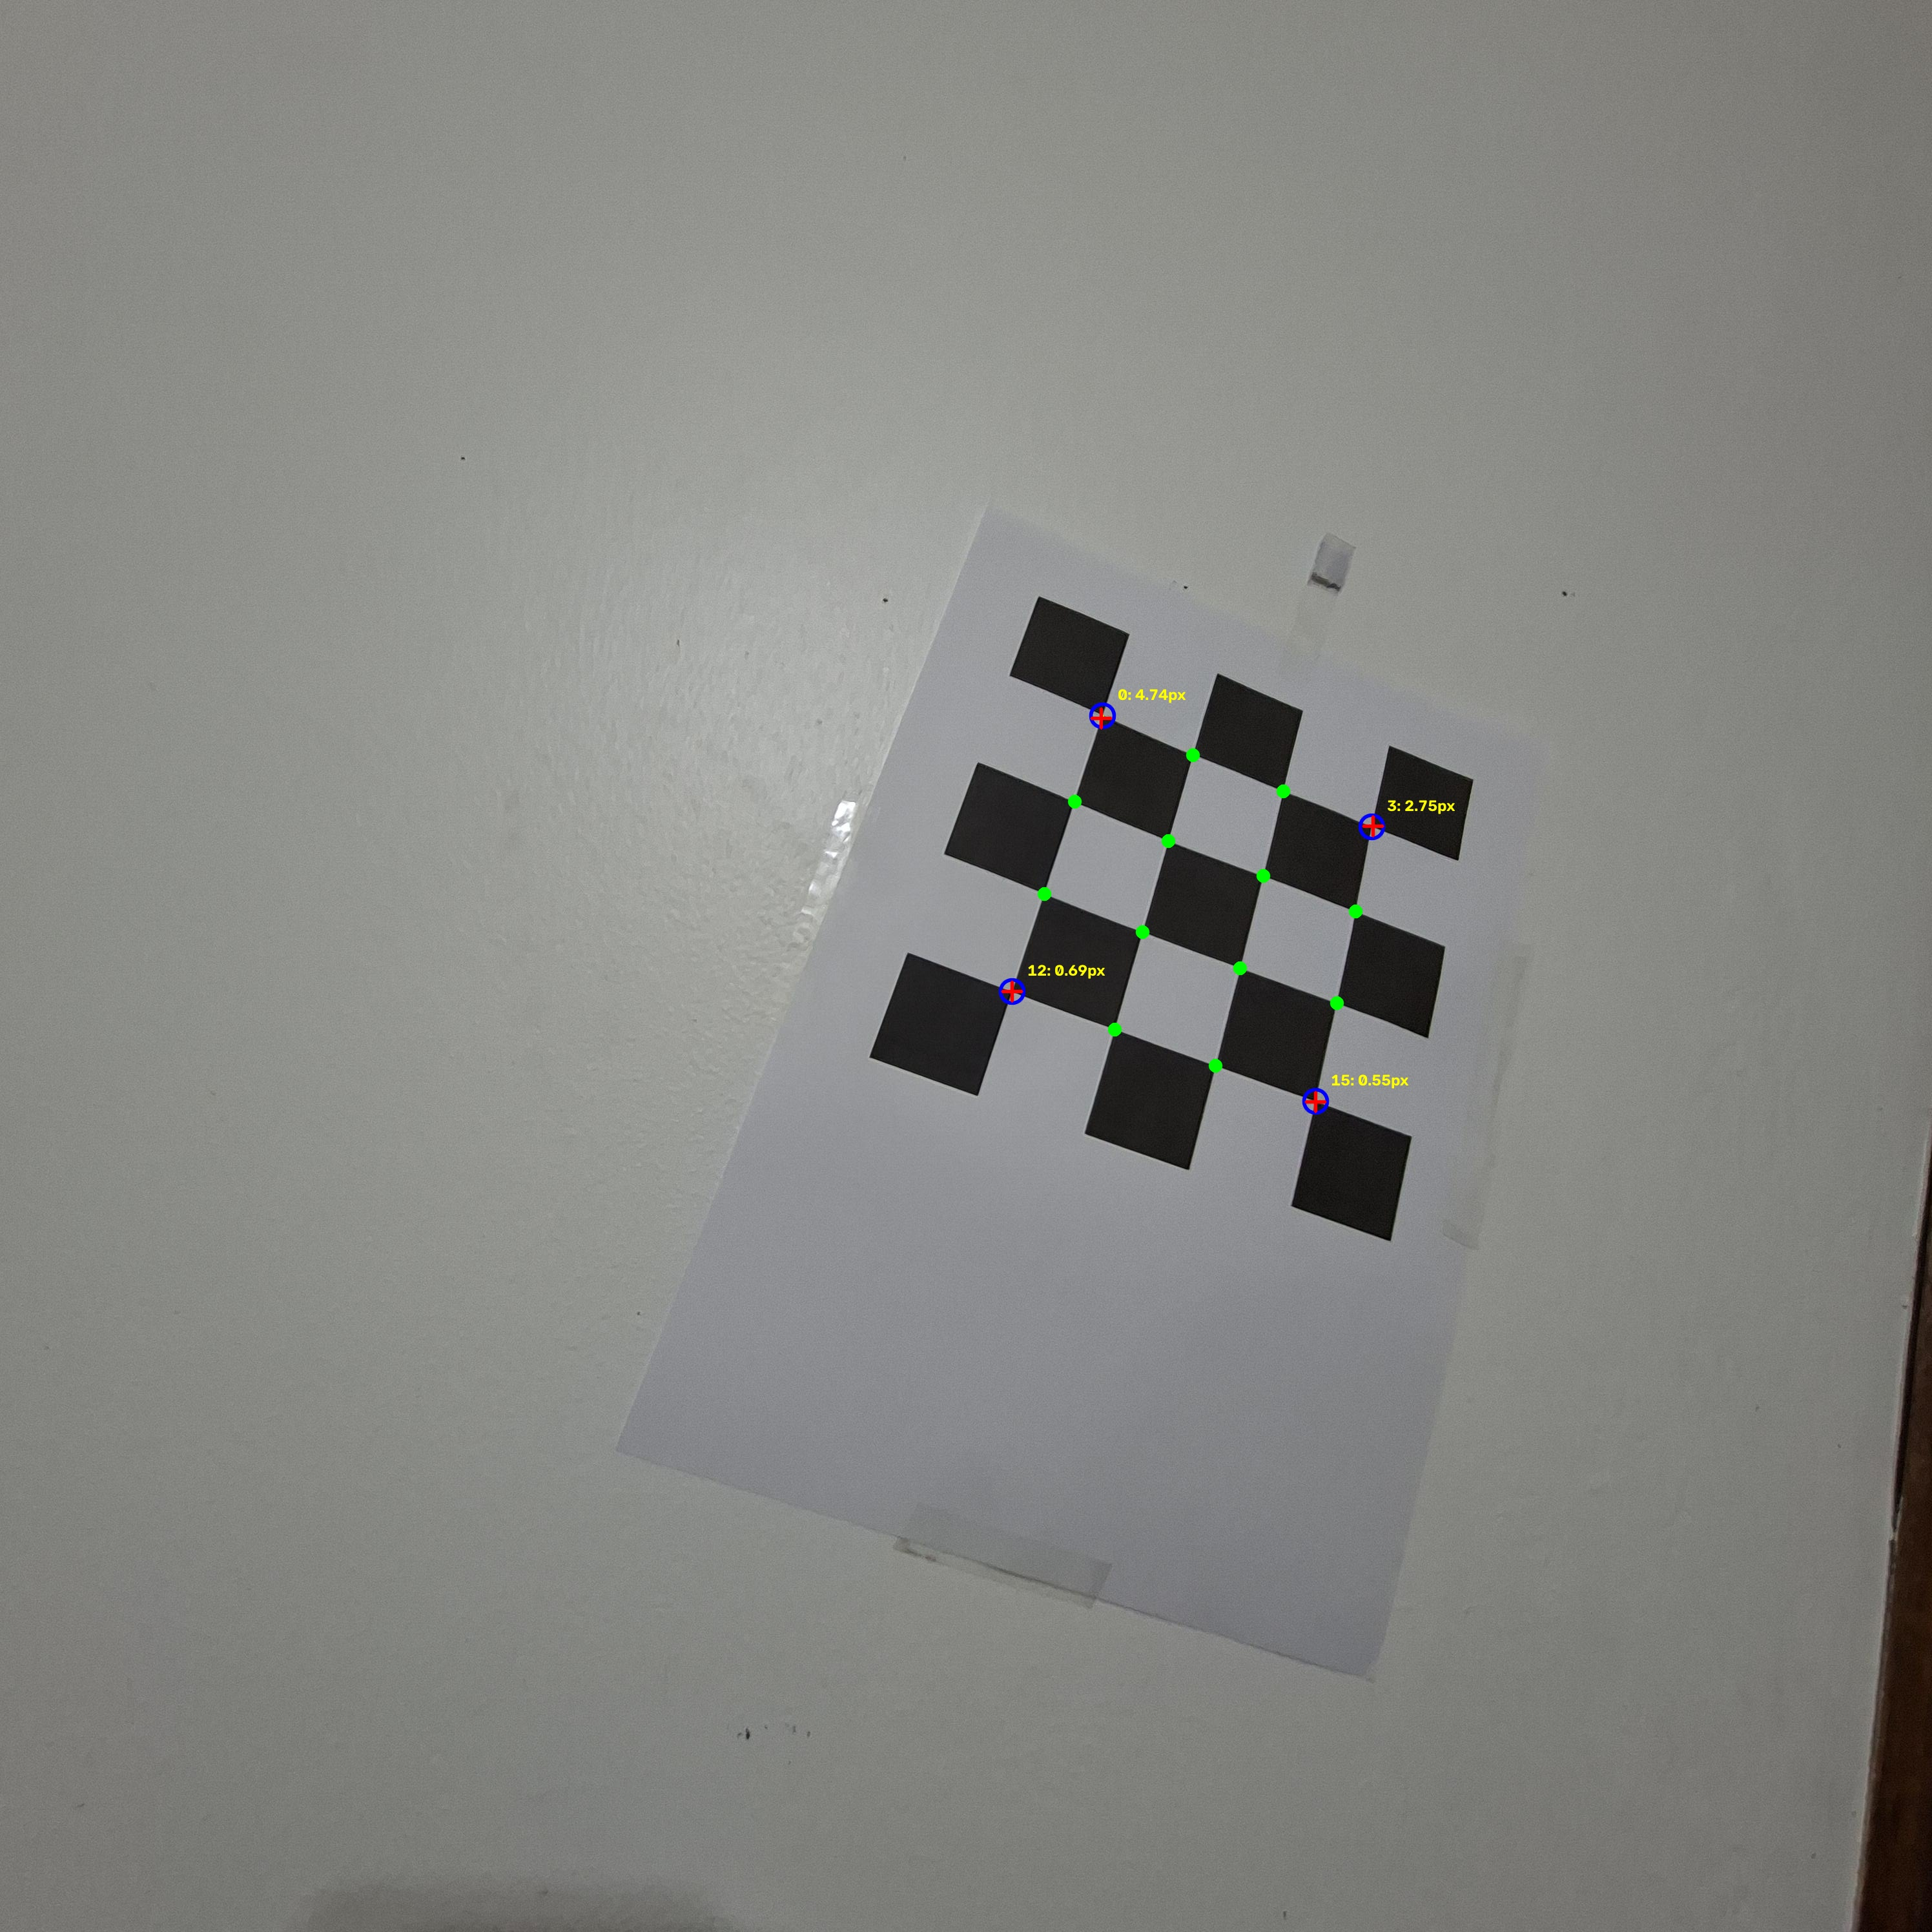
\includegraphics[height=5.5cm,trim=1367bp 1037bp 619bp 907bp,clip]{projection-cam05.jpg}
  \caption{Câmera 0,5x, fotografia inédita \texttt{002.jpg}, com a convenção da
  Figura~\ref{fig:projection1}. Média nesta imagem: $2{,}183$~px.
  As duas figuras foram enquadradas somente no documento.}
  \label{fig:projection05}
  \end{minipage}
\end{figure}

\FloatBarrier
Nas fotografias inéditas, o erro médio aumentou $153{,}19\%$ na câmera 1x
e $14{,}50\%$ na câmera 0,5x; o RMSE aumentou $157{,}75\%$ e $19{,}41\%$,
respectivamente. A câmera 0,5x apresentou menores erros nesse novo conjunto,
embora a câmera principal tivesse menores erros nas fotografias da calibração.
A escala e a posição do tabuleiro, sua inclinação e resíduos do modelo podem
influenciar a diferença; esses fatores não foram isolados.

As novas fotografias não participaram da calibração intrínseca, e os quatro
cantos reservados também não participaram da estimação da pose. A avaliação
verifica, portanto, a projeção em imagens inéditas, mas a pose de cada imagem
continua sendo estimada a partir de 12 correspondências conhecidas. Com apenas
três imagens por câmera, os resultados descrevem esta amostra e não estabelecem
uma superioridade geral de uma das câmeras.
